\section{RAG}
\label{sec:rag}

Retrieval Augmented Generation (RAG) adalah sebuah teknik dalam \textit{Artificial Intelligence} yang menggunakan \textit{Natural Language} untuk memperkaya \textit{Large Language Models} dengan pengetahuan eksternal. RAG muncul sebagai solusi dari kekurangan LLM yang selalu menjawab berdasarkan pengetahuan yang kurang relevan atau tidak lengkap. Pendekatan ini memungkinkan model untuk mengambil informasi yang relevan dari dokumen atau basis data tertentu saat berjalan, memperkuat pengetahuan internalnya dan meningkatkan akurasi serta relevansi responsnya \parencite{merritt2025rag}.

Istilah "RAG" pertama kali diperkenalkan oleh \cite{lewis2020retrieval} dari Facebook AI Research, University College London, dan New York University. Dalam makalah tersebut, Lewis dan timnya mengembangkan sebuah model RAG yang mengintegrasikan memori parametrik dan non-parametrik dalam proses generasi bahasa. Memori parametrik berupa model seq2seq (\textit{sequence-to-sequence}) yang telah dilatih sebelumnya, seperti BART, sedangkan memori non-parametrik adalah indeks vektor padat dari Wikipedia yang diakses melalui sistem pengambilan informasi \textit{neural}, seperti \textit{Dense Passage Retriever} (DPR).

\begin{figure}[ht]
  \centering
  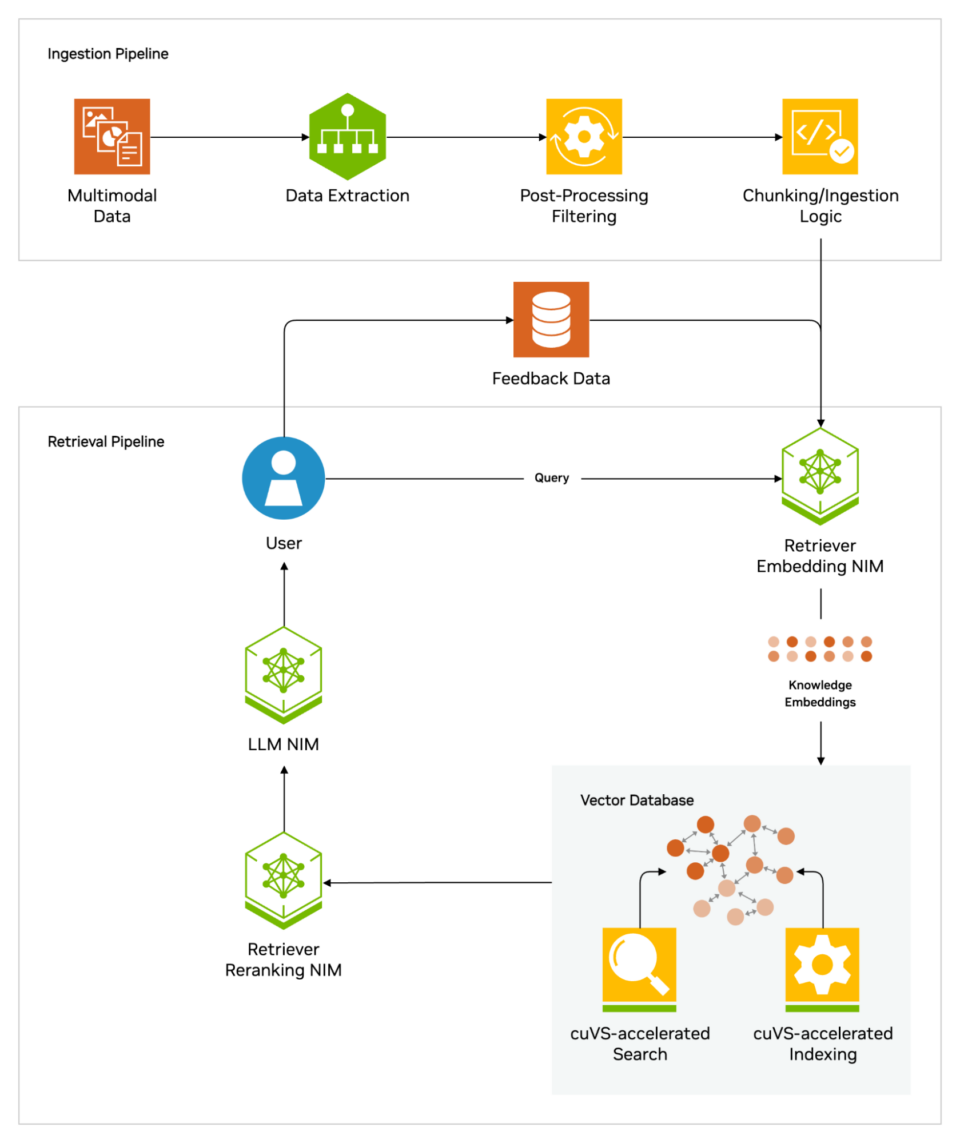
\includegraphics[width=0.7\textwidth]{resources/chapter-2/rag-overview.png}
  \caption{Gambaran umum cara kerja RAG \parencite{merritt2025rag}}
  \label{image:rag-overview}
\end{figure}

\begin{figure}[ht]
  \centering
  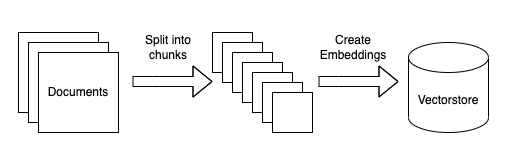
\includegraphics[width=0.7\textwidth]{resources/chapter-2/rag-ingestion.png}
  \caption{Diagram proses ingestion pada RAG \parencite{langchain_chatgpt_data}}
  \label{image:rag-ingestion}
  \end{figure}

\begin{figure}[ht]
  \centering
  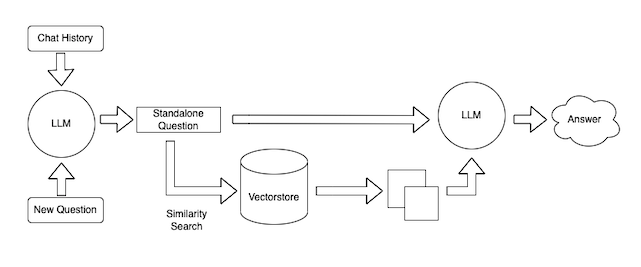
\includegraphics[width=0.7\textwidth]{resources/chapter-2/rag-query.png}
  \caption{Diagram proses query pada RAG \parencite{langchain_chatgpt_data}}
  \label{image:rag-query}
\end{figure}

Cara kerja dari RAG meliputi dua langkah utama, yaitu proses Data Ingestion dan Data Querying, yang dapat didekomposisi menjadi beberapa subproses. Data Ingestion melibatkan pengambilan data dari berbagai sumber, seperti dokumen atau basis data, dan mengubahnya menjadi format standar yang dapat diproses oleh model. Data Querying, di sisi lain, melibatkan pencarian data yang paling relevan dari sumber eksternal berdasarkan query yang diberikan. Proses ini memungkinkan model untuk mengakses informasi tambahan yang diperlukan untuk menghasilkan respons yang lebih akurat dan relevan. Berikut adalah penjelasan dari setiap subproses dalam RAG:

% \begin{enumerate}
%   \item Data Ingestion: Data dari berbagai sumber dimuat dan diubah menjadi format standar, seperti objek Dokumen LangChain, yang berisi teks dan metadata terkait.
%   \item Text Splitting: Teks yang dimuat dibagi menjadi potongan-potongan kecil untuk memastikan bahwa hanya bagian yang paling relevan yang disertakan dalam proses selanjutnya.
%   \item Embedding Creation: Setiap potongan teks diubah menjadi representasi numerik (\textit{embedding}) menggunakan model \textit{embedding}, memungkinkan perbandingan semantik antar potongan.
%   \item Embedding Storing in Vectorstore: \textit{Embedding} dan dokumen terkait disimpan dalam vectorstore, basis data yang memungkinkan pencarian cepat potongan teks yang paling relevan berdasarkan kesamaan semantik.
%   \item Document Retrieval: Saat menerima query, sistem mencari potongan teks yang paling relevan dari vectorstore dengan membandingkan \textit{embedding} query dengan \textit{embedding} yang ada.
%   \item Response Generation: Query dan dokumen yang diambil digabungkan dan diberikan ke LLM untuk menghasilkan respons yang informatif dan kontekstual.
% \end{enumerate}

\begin{enumerate}
  \item \textbf{Data Ingestion} \\
  Proses ini melibatkan pengolahan data menjadi format yang dapat digunakan oleh model bahasa. Proses ingesti dapat dibagi menjadi beberapa sub-langkah sebagai berikut:
  \begin{enumerate}
    \item \textbf{Load Data Sources to Text} \\
    Tahap ini melibatkan pemuatan data dari berbagai sumber (seperti PDF, dokumen, teks, dan lainnya) ke dalam format teks standar. Dalam implementasi LangChain, data dikonversi menjadi objek Document yang berisi teks dan metadata terkait dokumen tersebut.
    \item \textbf{Chunk Text} \\
    Teks yang telah dimuat kemudian dipecah menjadi potongan-potongan kecil (\textit{chunks}). Langkah ini penting karena model bahasa umumnya memiliki batas jumlah teks yang dapat diproses. Dengan membuat potongan teks sekecil mungkin, sistem dapat memilih hanya bagian yang paling relevan untuk digunakan.
    \item \textbf{Embed Text} \\
    Setiap potongan teks diubah menjadi \textit{embeddings} menggunakan model \textit{embedding} seperti OpenAI text-embedding-ada-002. \textit{Embeddings} ini memungkinkan sistem untuk menemukan potongan teks yang paling relevan berdasarkan kesamaan semantik, bukan sekadar kecocokan kata kunci.
    \item \textbf{Load Embeddings to Vectorstore} \\
    \textit{Embeddings} dan dokumen terkait kemudian disimpan dalam basis data vektor (vectorstore) seperti FAISS, Pinecone, atau Chroma. Vectorstore membantu dalam pencarian potongan teks yang paling mirip secara cepat dan efisien.
  \end{enumerate}
  \item \textbf{Data Querying} \\
  Proses ini melibatkan penggunaan data yang telah diingesti untuk menjawab pertanyaan pengguna. Proses kueri juga dapat dibagi menjadi beberapa sub-langkah:
  \begin{enumerate}
    \item \textbf{Combine Chat History and New Question} \\
    Sistem menggabungkan riwayat percakapan dengan pertanyaan baru menjadi sebuah pertanyaan mandiri (\textit{standalone question}). Langkah ini penting untuk memungkinkan pengguna mengajukan pertanyaan lanjutan tanpa harus mengulang konteks secara eksplisit.
    \item \textbf{Lookup Relevant Documents} \\
    Menggunakan \textit{embeddings} dan vectorstore yang dibuat selama proses ingesti, sistem mencari dokumen yang paling relevan dengan pertanyaan mandiri. Langkah ini memastikan bahwa hanya informasi yang relevan yang digunakan untuk menjawab pertanyaan.
    \item \textbf{Generate a Response} \\
    Pertanyaan mandiri dan dokumen relevan yang ditemukan kemudian dimasukkan ke dalam LLM untuk menghasilkan respons. Proses ini menggunakan prompt khusus yang disebut QA\_PROMPT, yang dapat disesuaikan untuk memberikan gaya percakapan tertentu pada \textit{chatbot}.
  \end{enumerate}
\end{enumerate}

RAG telah menjadi pendekatan yang sangat populer sejak diperkenalkan untuk meningkatkan kemampuan LLM dalam mengakses dan memanfaatkan informasi dari data internal tanpa perlu melakukan \textit{fine-tuning} model. Dengan menggunakan RAG, aplikasi dapat menjawab pertanyaan berdasarkan dokumen perusahaan, basis pengetahuan, atau \textit{dataset} spesifik domain dengan akurasi yang lebih tinggi dan risiko halusinasi yang lebih rendah.

Implementasi RAG dapat dilakukan menggunakan \textit{framework} seperti LangChain yang menyediakan komponen modular untuk membangun \textit{pipeline} RAG. LangChain menyediakan \textit{interface} sederhana untuk berinteraksi dengan \textit{chatbot} melalui terminal (CLI) dan juga memungkinkan \textit{deployment} menggunakan Gradio untuk \textit{interface} web. Dengan pendekatan modular ini, setiap komponen dalam \textit{text} RAG dapat disesuaikan atau diganti sesuai dengan kebutuhan spesifik aplikasi.